\documentclass[12pt,a4paper]{article}
\usepackage[polish]{babel}
\usepackage[T1]{fontenc}
\usepackage{hyperref}
\usepackage{url}
\usepackage{graphicx}
\graphicspath{ {images/} }
\usepackage{csquotes}
\usepackage[utf8x]{inputenc}
\usepackage{fancyvrb}

\addtolength{\hoffset}{-1.5cm}
\addtolength{\marginparwidth}{-1.5cm}
\addtolength{\textwidth}{3cm}
\addtolength{\voffset}{-1cm}
\addtolength{\textheight}{2.5cm}
\setlength{\topmargin}{0cm}
\usepackage{algorithm}
\usepackage[noend]{algpseudocode}
\setlength{\headheight}{0cm}

\begin{document}
    \begin{titlepage}
       \begin{center}
           \vspace*{1cm}
           
           {\fontsize{23}{25}\selectfont Dokumentacja projektu\\Bazy Danych}
     
            \vspace{1.0cm}
        
            {\fontsize{17}{18}\selectfont Dawid Bitner \\ Marcin Krupa}
           
            \vspace{0.4cm}
           
            {\fontsize{12}{13}\selectfont 1 lipca 2019}
           
            \vfill
            \vspace{0.8cm}
     
            {\fontsize{13}{14}\selectfont Politechnika Śląska\\Wydział Matematyki Stosowanej\\Rok akademicki 2018/2019}
     
       \end{center}
    \end{titlepage}
	\newpage
	\tableofcontents
	\newpage
	\section{Część I}
	\subsection{Opis projektu}
        Baza danych została stworzona dla aplikacji, której zadaniem jest obsługa zdarzeń związanych z rozgrywkami polskiej Ekstraklasy w piłce nożnej. Cały projekt jest wzorowany na systemie \textit{EXTRANET}  z którego korzystają trenerzy, delegaci, oraz sędziowie w celu obsługi rozgrywek. Baza posiada takie tabele jak: kluby, piłkarze, trenerzy, stadiony, czy informacje dotyczące strojów. Dodatkowo została stworzona tabela przechowująca informacje o logowaniu użytkowników.
        
    \section{Część II}
    \subsection{Diagram związków encji}
        \begin{center}
            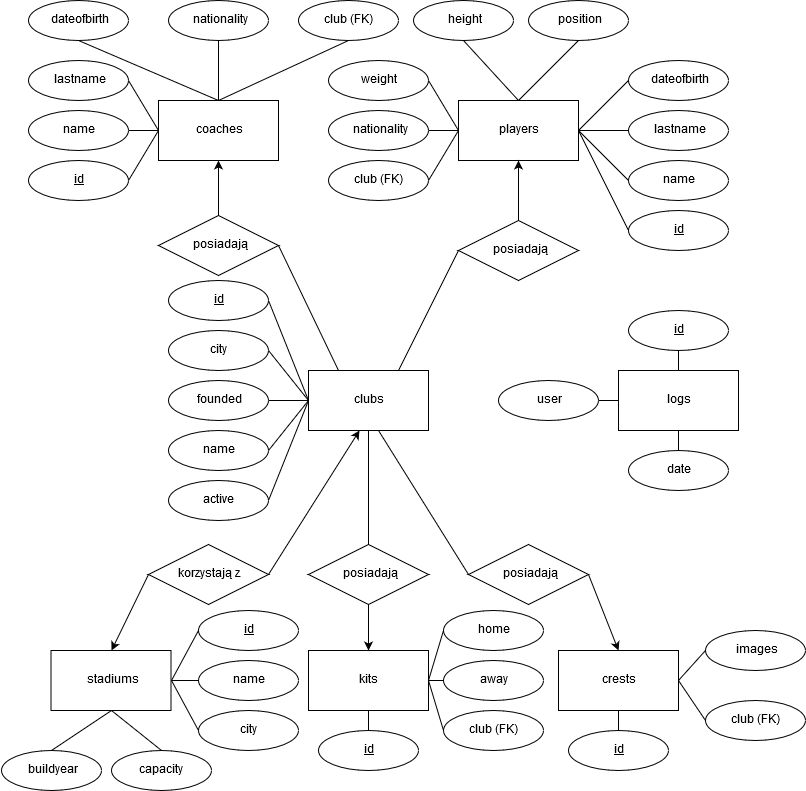
\includegraphics[scale=0.5]{diagram.png}
        \end{center}
    
    \subsection{Model relacyjny}
        \begin{center}
            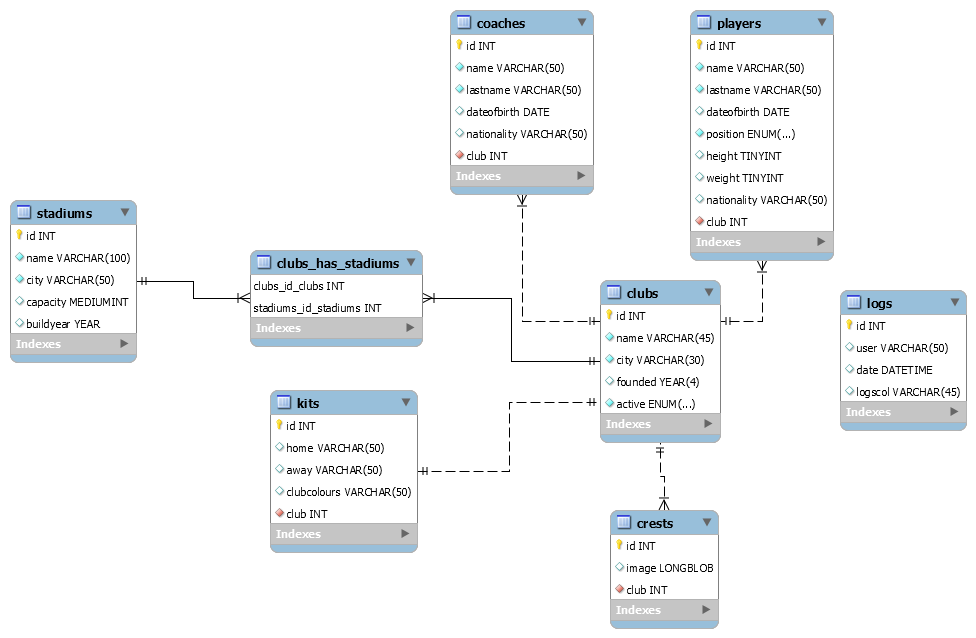
\includegraphics[scale=0.5]{database-schema.png}
        \end{center}
    
    \newpage
    \section{Część III}
    \subsection{Instrukcja użytkowania}
    Program został stworzony z myślą o wykorzystaniu go przez użytkowników dwóch typów kont: administratora oraz zwykłego użytkownika. Każdy z tych typów kont zapewnia inną funkcjonalność, która została odzwierciedlona w programie.
    
    Aby prawidłowo korzystać z funkcjonalności programu, należy mieć połączenie z Internetem. Po uruchomieniu programu z pliku $application.exe$ użytkownikowi pojawi się ekran logowania.
    
    \begin{center}
        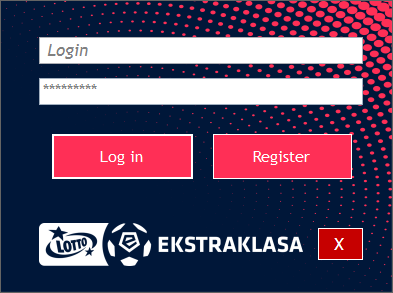
\includegraphics[scale=1]{login-panel.png}
        \begin{flushleft}
            \begin{scriptsize}
            \begin{list}{}{\leftmargin=21.5em}\raggedright\item\relax
            Rysunek 1: Ekran logowania.
            \end{list}
            \end{scriptsize}
        \end{flushleft}
    \end{center}
    
    Użytkownik, według założeń projektu, ma możliwość wyłącznie przeglądania rekordów w bazie. Administrator natomiast posiada niemal pełną kontrolę nad bazą. W zależności od tego na jaki typ konta zaloguje się użytkownik, pojawi mu się inna forma z programem, różniąca się przede kontrolką umożliwiającą przełączanie się pomiędzy panelami.
    
    \begin{center}
        
\includegraphics[scale=1]{admin-controls.png}
        \begin{flushleft}
            \begin{scriptsize}
            \begin{list}{}{\leftmargin=19em}\raggedright\item\relax
            Rysunek 2: Kontrolka administratora.
            \end{list}
            \end{scriptsize}
        \end{flushleft}
    \end{center}
    
    Kontrolki kolejno od lewej do prawej oznaczają:
    \begin{itemize}
        \item wybór panelu wyszukiwania,
        \item wybór panelu wprowadzania rekordów do tabeli,
        \item wybór panelu usuwania rekordu z tabeli,
        \item wybór panelu aktualizacji rekordu w tabeli.
    \end{itemize}
    
    \subsubsection{Panel wyszukiwania}
    Panel ten jest dostępny zarówno dla administratora jak i użytkownika.
    \begin{center}
        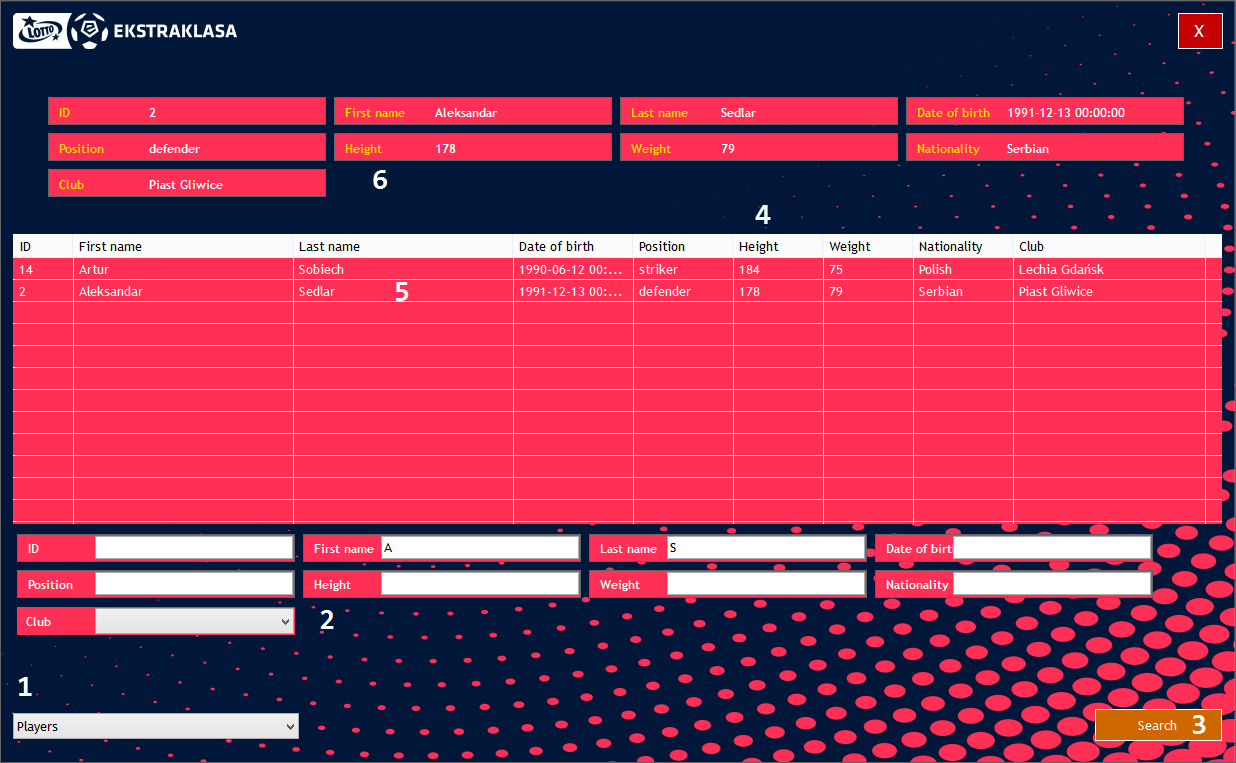
\includegraphics[scale=0.47]{select-panel.png}
        \begin{flushleft}
            \begin{scriptsize}
            \begin{list}{}{\leftmargin=13.5em}\raggedright\item\relax
            Rysunek 3: Panel wyszukiwania z przykładowym wynikiem zapytania.
            \end{list}
            \end{scriptsize}
        \end{flushleft}
    \end{center}
    
    Aby wyszukiwać rekordy w bazie:
    \begin{enumerate}
        \item Należy wybrać tabele z której chcemy wyszukiwać nasze rekordy z rozwijanej listy z tabelami.
        \item Następnie określamy kryteria zapytań. Krok ten można pominąć jeśli chcemy wyświetlić wszystkie rekordy w tabeli.
        \item Naciskając przycisk $Search$ wyszukujemy rekordy w bazie. Jeśli użytkownik nie określił tabeli z której chce wyszukiwać rekordy, nic się nie wydarzy.
        \item Wyświetlone rekordy można sortować. W tym celu należy kliknąć w nazwę kolumny (na powyższym przykładzie pokazano sortowanie po kolumnie $Height$).
        \item Naciskając dwukrotnie w rekord wyświetlą nam się nad tabelą dane dotyczące konkretnego elementu.
        \item Dane dotyczące rekordu wskazanego dwuklikiem.
    \end{enumerate}
    
    \newpage
    
    \subsubsection{Panel wprowadzania rekordów do tabeli}
    Dostępny tylko dla administratora, umożliwia wprowadzanie rekordów do wybranej tabeli.
    \begin{center}
        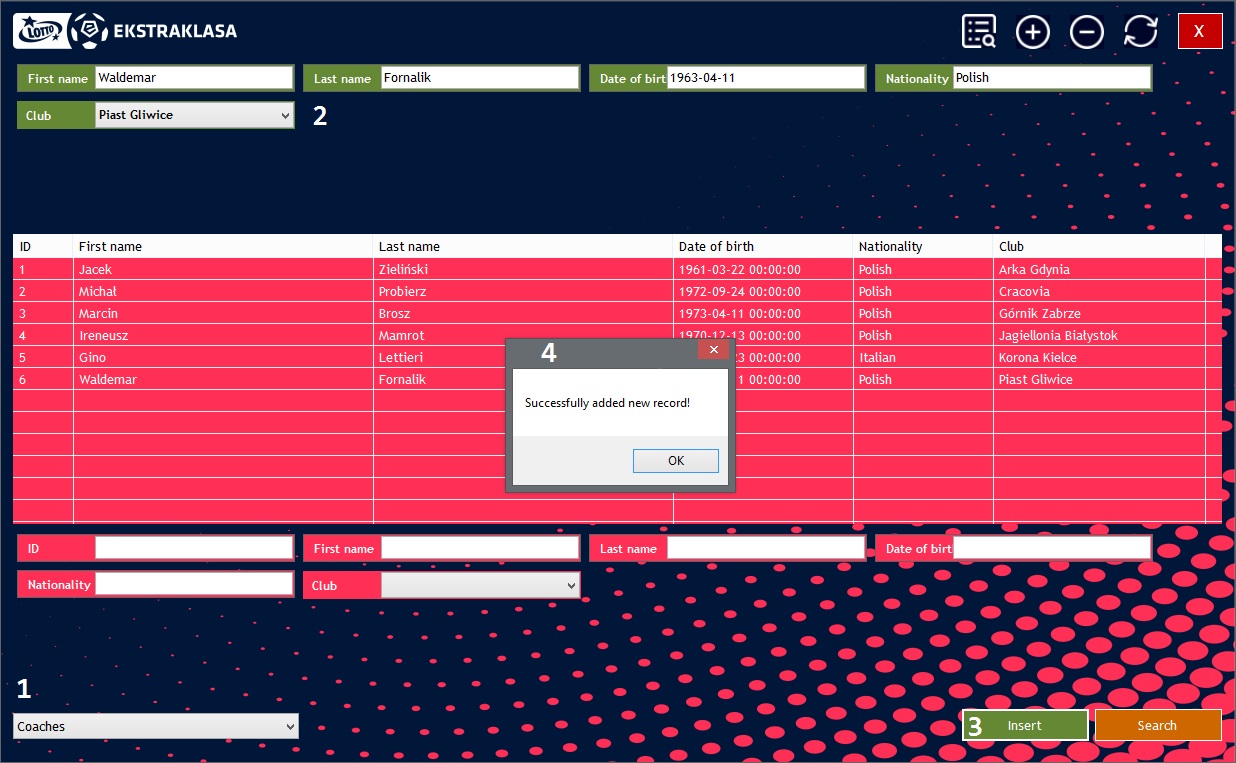
\includegraphics[scale=0.47]{insert-panel.png}
        \begin{flushleft}
            \begin{scriptsize}
            \begin{list}{}{\leftmargin=13.5em}\raggedright\item\relax
            Rysunek 4: Panel wprowadzania rekordów do tabeli, z przykładowym trenerem.
            \end{list}
            \end{scriptsize}
        \end{flushleft}
    \end{center}
    
    Aby wprowadzać rekordy do tabeli:
    \begin{enumerate}
        \item Należy wybrać tabele do której chcemy wprowadzać nowe rekordy z rozwijalnej listy.
        \item Ukażą się nam u góry kontrolki z miejscem na wpisanie nowego rekordu w tabeli. Dla ułatwienia w dalszym ciągu można wyszukiwać rekordy w tabeli.
        \item Naciskając przycisk $Insert$ zatwierdzamy wprowadzenie rekordu do tabeli. Ważnym jest, aby były wprowadzone wszystkie dane. W innym przypadku użytkownik zostanie powiadomiony o ich braku.
        \item Po akcji wprowadzenia rekordu do tabeli, użytkownik zostaje powiadomiony o udanej lub nieudanej próbie wprowadzenia rekordu do tabeli.
    \end{enumerate}
    
    \newpage
    
    \subsubsection{Panel usuwania rekordu w tabeli}
    Dostępny tylko dla administratora, umożliwia usuwanie pojedynczego rekordu z tabeli.
    \begin{center}
        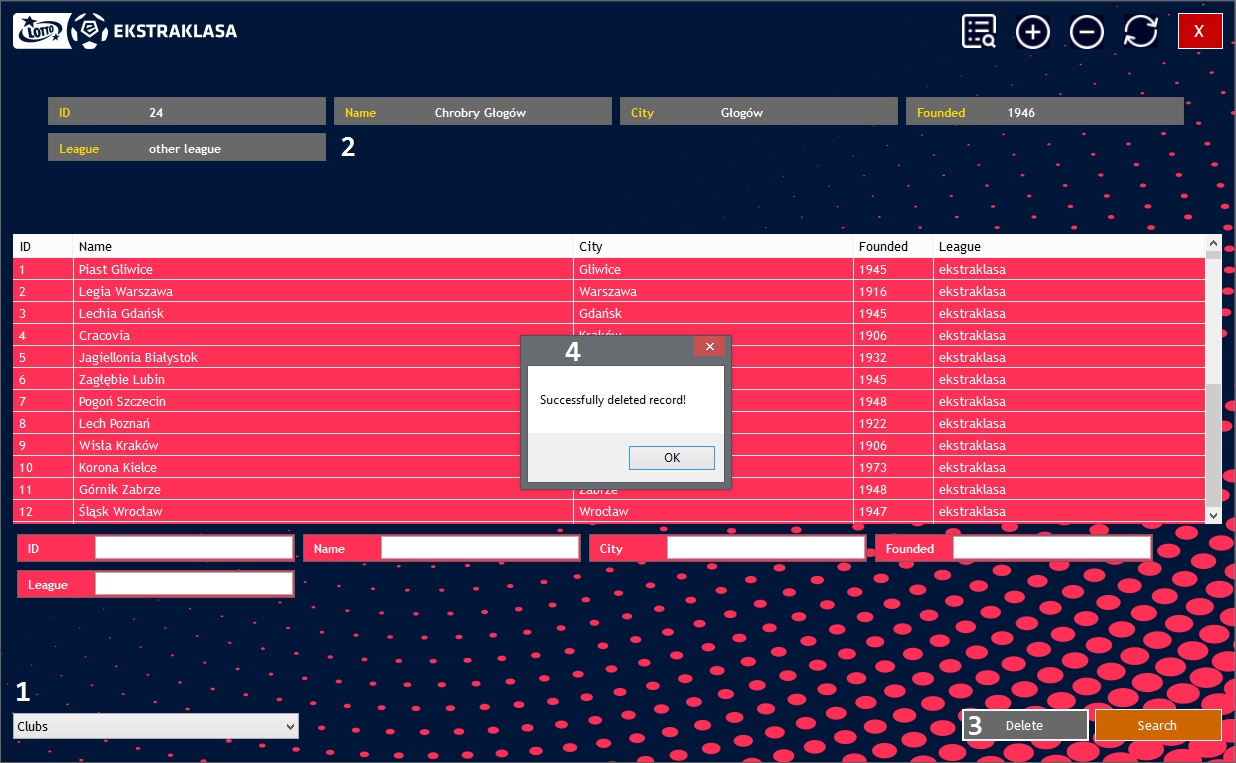
\includegraphics[scale=0.47]{delete-panel.png}
        \begin{flushleft}
            \begin{scriptsize}
            \begin{list}{}{\leftmargin=13.5em}\raggedright\item\relax
            Rysunek 5: Panel usuwania rekordu z tabeli, z przykładowym klubem.
            \end{list}
            \end{scriptsize}
        \end{flushleft}
    \end{center}
    
    Aby usuwać rekordy z tabeli:
    \begin{enumerate}
        \item Należy wybrać tabele z której chcemy usunąć wybrany rekord z rozwijalnej listy.
        \item Naciskając dwukrotnie w rekord wyświetlą nam się nad tabelą dane dotyczące tego rekordu. Dopiero wykonując te czynność określamy jaki element chcemy usunąć z tabeli.
        \item Naciskając przycisk $Delete$ zatwierdzamy usunięcie rekordu z tabeli.
        \item Po akcji usunięcia rekordu z tabeli, użytkownik zostaje powiadomiony o udanej lub nieudanej próbie usunięcia rekordu z tabeli.
    \end{enumerate}
    
    \newpage
    
    \subsubsection{Panel edytowania rekordu w tabeli}
    Dostępny tylko dla administratora, umożliwia edytowanie pojedynczego rekordu z tabeli.
    \begin{center}
        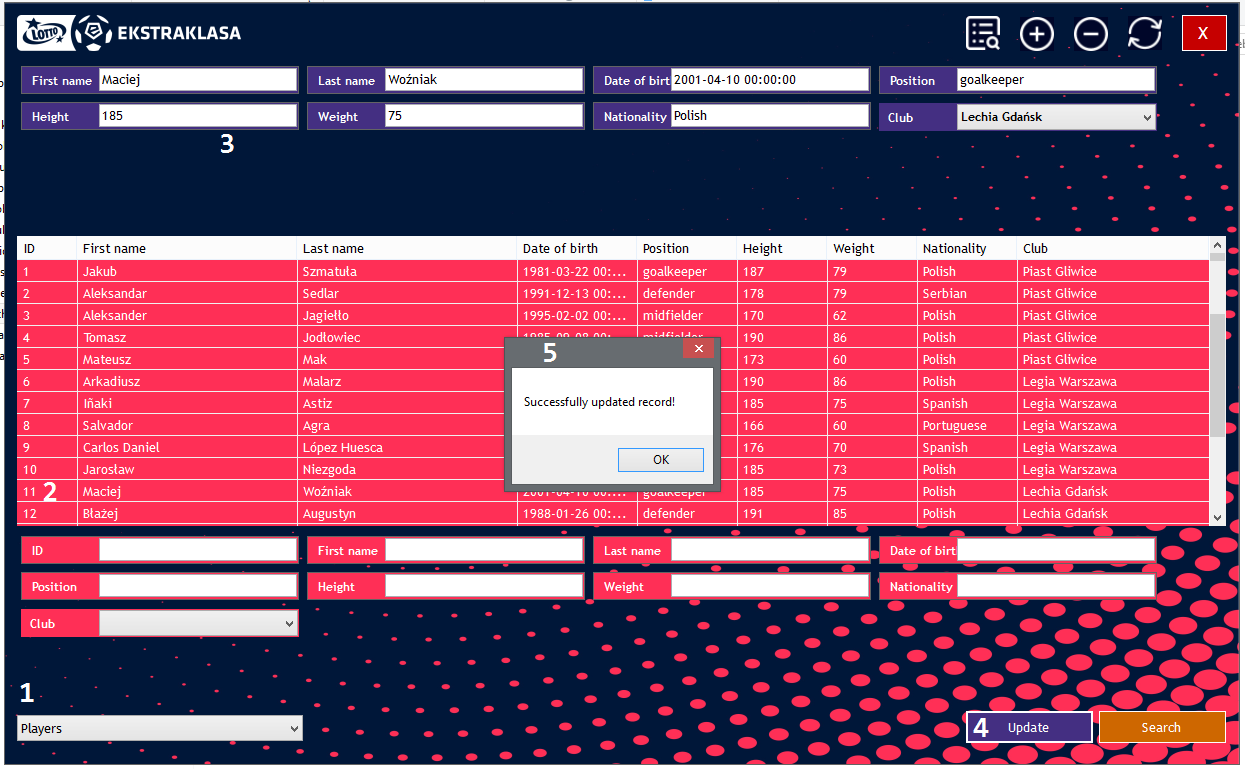
\includegraphics[scale=0.47]{update-panel.png}
        \begin{flushleft}
            \begin{scriptsize}
            \begin{list}{}{\leftmargin=13.5em}\raggedright\item\relax
            Rysunek 6: Panel edytowania rekordu w tabeli, z przykładowym graczem.
            \end{list}
            \end{scriptsize}
        \end{flushleft}
    \end{center}
    
    Aby usuwać rekordy z tabeli:
    \begin{enumerate}
        \item Należy wybrać tabele w której chcemy edytować wybrany rekord z rozwijalnej listy.
        \item Naciskając dwukrotnie w rekord wyświetlą nam się nad tabelą dane dotyczące tego rekordu. Dopiero wykonując te czynność określamy jaki element chcemy edytować w tabeli.
        \item Edytujemy dane rekordu z tabeli. 
        \item Naciskając przycisk $Update$ zatwierdzamy edycje rekordu z tabeli. Ważnym jest, aby były wprowadzone wszystkie dane. W innym przypadku użytkownik zostanie powiadomiony o ich braku.
        \item Po akcji edytowania rekordu w tabeli, użytkownik zostaje powiadomiony o udanej lub nieudanej próbie edytowania rekordu w tabeli.
    \end{enumerate}
    
    \newpage
    \section{Część IV}
    \subsection{Kod tworzący tabele}
    \begin{verbatim}
SET SQL_MODE = "NO_AUTO_VALUE_ON_ZERO";
SET AUTOCOMMIT = 0;
START TRANSACTION;
SET time_zone = "+00:00";


/*!40101 SET @OLD_CHARACTER_SET_CLIENT=@@CHARACTER_SET_CLIENT */;
/*!40101 SET @OLD_CHARACTER_SET_RESULTS=@@CHARACTER_SET_RESULTS */;
/*!40101 SET @OLD_COLLATION_CONNECTION=@@COLLATION_CONNECTION */;
/*!40101 SET NAMES utf8mb4 */;

--
-- Baza danych: `ekstraklasa`
--

-- --------------------------------------------------------

--
-- Struktura tabeli dla tabeli `clubs`
--

CREATE TABLE `clubs` (
  `id` int(10) UNSIGNED NOT NULL,
  `name` varchar(50) COLLATE utf8mb4_unicode_ci NOT NULL,
  `city` varchar(50) COLLATE utf8mb4_unicode_ci NOT NULL,
  `founded` year(4) DEFAULT NULL,
  `active` enum('ekstraklasa','other league','doesn''t exist') 
  COLLATE utf8mb4_unicode_ci NOT NULL
) ENGINE=InnoDB DEFAULT CHARSET=utf8mb4 COLLATE=utf8mb4_unicode_ci;

--
-- Struktura tabeli dla tabeli `clubs_has_stadiums`
--

CREATE TABLE `clubs_has_stadiums` (
  `clubs_id_clubs` int(10) UNSIGNED NOT NULL,
  `stadiums_id_stadiums` int(10) UNSIGNED NOT NULL
) ENGINE=InnoDB DEFAULT CHARSET=utf8mb4 COLLATE=utf8mb4_unicode_ci;

--
-- Struktura tabeli dla tabeli `coaches`
--

CREATE TABLE `coaches` (
  `id` int(10) UNSIGNED NOT NULL,
  `name` varchar(50) COLLATE utf8mb4_unicode_ci NOT NULL,
  `lastname` varchar(50) COLLATE utf8mb4_unicode_ci NOT NULL,
  `dateofbirth` date DEFAULT NULL,
  `nationality` varchar(50) COLLATE utf8mb4_unicode_ci DEFAULT NULL,
  `club` int(10) UNSIGNED NOT NULL
) ENGINE=InnoDB DEFAULTCHARSET=utf8mb4 COLLATE=utf8mb4_unicode_ci;

--
-- Struktura tabeli dla tabeli `crests`
--

CREATE TABLE `crests` (
  `id` int(10) UNSIGNED NOT NULL,
  `image` longblob,
  `club` int(10) UNSIGNED NOT NULL
) ENGINE=InnoDB DEFAULT CHARSET=utf8mb4 COLLATE=utf8mb4_unicode_ci;

--
-- Struktura tabeli dla tabeli `kits`
--

CREATE TABLE `kits` (
  `id` int(10) UNSIGNED NOT NULL,
  `home` varchar(50) COLLATE utf8mb4_unicode_ci DEFAULT NULL,
  `away` varchar(50) COLLATE utf8mb4_unicode_ci DEFAULT NULL,
  `clubcolours` varchar(50) COLLATE utf8mb4_unicode_ci DEFAULT NULL,
  `club` int(10) UNSIGNED NOT NULL
) ENGINE=InnoDB DEFAULT CHARSET=utf8mb4 COLLATE=utf8mb4_unicode_ci;

--
-- Struktura tabeli dla tabeli `logs`
--

CREATE TABLE `logs` (
  `id` int(11) NOT NULL,
  `user` varchar(40) COLLATE utf8mb4_unicode_ci NOT NULL,
  `date` datetime NOT NULL
) ENGINE=InnoDB DEFAULT CHARSET=utf8mb4 COLLATE=utf8mb4_unicode_ci;

--
-- Struktura tabeli dla tabeli `players`
--

CREATE TABLE `players` (
  `id` int(10) UNSIGNED NOT NULL,
  `name` varchar(50) COLLATE utf8mb4_unicode_ci NOT NULL,
  `lastname` varchar(50) COLLATE utf8mb4_unicode_ci NOT NULL,
  `dateofbirth` date DEFAULT NULL,
  `position` enum('goalkeeper','defender','midfielder','striker') 
  COLLATE utf8_polish_ci NOT NULL,
  `height` tinyint(3) UNSIGNED DEFAULT NULL,
  `weight` tinyint(3) UNSIGNED DEFAULT NULL,
  `nationality` varchar(50) COLLATE utf8mb4_unicode_ci DEFAULT NULL,
  `club` int(10) UNSIGNED NOT NULL
) ENGINE=InnoDB DEFAULT CHARSET=utf8mb4 COLLATE=utf8mb4_unicode_ci;

--
-- Struktura tabeli dla tabeli `stadiums`
--

CREATE TABLE `stadiums` (
  `id` int(10) UNSIGNED NOT NULL,
  `name` varchar(100) COLLATE utf8mb4_unicode_ci NOT NULL,
  `city` varchar(50) COLLATE utf8mb4_unicode_ci NOT NULL,
  `capacity` mediumint(8) UNSIGNED DEFAULT NULL,
  `buildyear` year(4) DEFAULT NULL
) ENGINE=InnoDB DEFAULT CHARSET=utf8mb4 COLLATE=utf8mb4_unicode_ci;

--
-- Indeksy dla zrzutów tabel
--

--
-- Indeksy dla tabeli `clubs`
--
ALTER TABLE `clubs`
  ADD PRIMARY KEY (`id`),
  ADD UNIQUE KEY `id_clubs_UNIQUE` (`id`),
  ADD UNIQUE KEY `name_clubs_UNIQUE` (`name`);

--
-- Indeksy dla tabeli `clubs_has_stadiums`
--
ALTER TABLE `clubs_has_stadiums`
  ADD PRIMARY KEY (`clubs_id_clubs`,`stadiums_id_stadiums`),
  ADD KEY `clubs_has_stadiums_stadiums_idx` (`stadiums_id_stadiums`),
  ADD KEY `clubs_has_stadiums_clubs_idx` (`clubs_id_clubs`);

--
-- Indeksy dla tabeli `coaches`
--
ALTER TABLE `coaches`
  ADD PRIMARY KEY (`id`),
  ADD KEY `coaches_clubs_idx` (`club`);

--
-- Indeksy dla tabeli `crests`
--
ALTER TABLE `crests`
  ADD PRIMARY KEY (`id`),
  ADD UNIQUE KEY `id_crests_UNIQUE` (`id`),
  ADD KEY `crests_clubs_idx` (`club`);

--
-- Indeksy dla tabeli `kits`
--
ALTER TABLE `kits`
  ADD PRIMARY KEY (`id`),
  ADD UNIQUE KEY `id_kits_UNIQUE` (`id`),
  ADD UNIQUE KEY `club_UNIQUE` (`club`),
  ADD KEY `kits_clubs_idx` (`club`);

--
-- Indeksy dla tabeli `logs`
--
ALTER TABLE `logs`
  ADD PRIMARY KEY (`id`);

--
-- Indeksy dla tabeli `players`
--
ALTER TABLE `players`
  ADD PRIMARY KEY (`id`),
  ADD UNIQUE KEY `id_players_UNIQUE` (`id`),
  ADD KEY `players_clubs_idx` (`club`);

--
-- Indeksy dla tabeli `stadiums`
--
ALTER TABLE `stadiums`
  ADD PRIMARY KEY (`id`),
  ADD UNIQUE KEY `id_stadiums_UNIQUE` (`id`);

--
-- AUTO_INCREMENT for dumped tables
--

--
-- AUTO_INCREMENT dla tabeli `clubs`
--
ALTER TABLE `clubs`
  MODIFY `id` int(10) UNSIGNED NOT NULL AUTO_INCREMENT, AUTO_INCREMENT=22;

--
-- AUTO_INCREMENT dla tabeli `coaches`
--
ALTER TABLE `coaches`
  MODIFY `id` int(10) UNSIGNED NOT NULL AUTO_INCREMENT, AUTO_INCREMENT=6;

--
-- AUTO_INCREMENT dla tabeli `crests`
--
ALTER TABLE `crests`
  MODIFY `id` int(10) UNSIGNED NOT NULL AUTO_INCREMENT, AUTO_INCREMENT=22;

--
-- AUTO_INCREMENT dla tabeli `kits`
--
ALTER TABLE `kits`
  MODIFY `id` int(10) UNSIGNED NOT NULL AUTO_INCREMENT, AUTO_INCREMENT=22;

--
-- AUTO_INCREMENT dla tabeli `logs`
--
ALTER TABLE `logs`
  MODIFY `id` int(11) NOT NULL AUTO_INCREMENT, AUTO_INCREMENT=12;

--
-- AUTO_INCREMENT dla tabeli `players`
--
ALTER TABLE `players`
  MODIFY `id` int(10) UNSIGNED NOT NULL AUTO_INCREMENT, AUTO_INCREMENT=16;

--
-- AUTO_INCREMENT dla tabeli `stadiums`
--
ALTER TABLE `stadiums`
  MODIFY `id` int(10) UNSIGNED NOT NULL AUTO_INCREMENT, AUTO_INCREMENT=8;

--
-- Ograniczenia dla zrzutów tabel
--

--
-- Ograniczenia dla tabeli `clubs_has_stadiums`
--
ALTER TABLE `clubs_has_stadiums`
  ADD CONSTRAINT `clubs_has_stadiums_clubs` FOREIGN KEY (`clubs_id_clubs`) 
  REFERENCES `clubs` (`id`),
  ADD CONSTRAINT `clubs_has_stadiums_stadiums` FOREIGN KEY (`stadiums_id_stadiums`) 
  REFERENCES `stadiums` (`id`);

--
-- Ograniczenia dla tabeli `coaches`
--
ALTER TABLE `coaches`
  ADD CONSTRAINT `coaches_clubs` FOREIGN KEY (`club`) REFERENCES `clubs` (`id`);

--
-- Ograniczenia dla tabeli `crests`
--
ALTER TABLE `crests`
  ADD CONSTRAINT `crests_clubs` FOREIGN KEY (`club`) REFERENCES `clubs` (`id`);

--
-- Ograniczenia dla tabeli `kits`
--
ALTER TABLE `kits`
  ADD CONSTRAINT `kits_clubs` FOREIGN KEY (`club`) REFERENCES `clubs` (`id`);

--
-- Ograniczenia dla tabeli `players`
--
ALTER TABLE `players`
  ADD CONSTRAINT `players_clubs` FOREIGN KEY (`club`) REFERENCES `clubs` (`id`);
COMMIT;

/*!40101 SET CHARACTER_SET_CLIENT=@OLD_CHARACTER_SET_CLIENT */;
/*!40101 SET CHARACTER_SET_RESULTS=@OLD_CHARACTER_SET_RESULTS */;
/*!40101 SET COLLATION_CONNECTION=@OLD_COLLATION_CONNECTION */;

    \end{verbatim}{}
    
    \subsection{Kod tworzący użytkowników}
    Z kodu zostały usunięte hasła.
    \begin{verbatim}
CREATE USER 'admin'@'localhost' IDENTIFIED VIA mysql_native_password USING '***';
GRANT USAGE ON *.* TO 'admin'@'localhost' REQUIRE NONE WITH MAX_QUERIES_PER_HOUR 
0 MAX_CONNECTIONS_PER_HOUR 0 MAX_UPDATES_PER_HOUR 0 MAX_USER_CONNECTIONS 0;
GRANT SELECT, INSERT, UPDATE, DELETE ON `ekstraklasa`.* TO 'admin'@'localhost';

CREATE USER 'user'@'localhost' IDENTIFIED VIA mysql_native_password USING '***';
GRANT USAGE ON *.* TO 'user'@'localhost' REQUIRE NONE WITH MAX_QUERIES_PER_HOUR 0 
MAX_CONNECTIONS_PER_HOUR 0 MAX_UPDATES_PER_HOUR 0 MAX_USER_CONNECTIONS 0;
GRANT SELECT ON `ekstraklasa`.* TO 'user'@'localhost';

GRANT USAGE ON *.* TO 'admin'@'localhost' IDENTIFIED BY PASSWORD '***';

GRANT SELECT, INSERT, UPDATE, DELETE ON `ekstraklasa`.* TO 'admin'@'localhost';

GRANT USAGE ON *.* TO 'user'@'localhost' IDENTIFIED BY PASSWORD '***';

GRANT SELECT ON `ekstraklasa`.* TO 'user'@'localhost';
\end{verbatim}{}

    \subsection{Funkcje i wyzwalacze}
    Funkcja, która formatuje przekazany łańcuch znaków tak, by wyrazy wewnątrz rozpoczynały się z wielkiej litery.
    
    Ustawia łańcuch znaków $res(result)$ jako wielka litera dla pierwszej wartości w łańcuchu wejściowym, łańcuch znaków $base$ jako reszta łańcucha wejściowego z użyciem funkcji $lower$ oraz indeks $i$ jako indeks pierwszego wystąpienia spacji w łańcuchu $base$.
    
    Następnie w pętli, która wykonuje się dopóki nie znajdzie w łańcuchu base kolejnej spacji, ustawia zmienną pomocniczą $x$ jako łańcuch znaków od pierwszej wartości z łańcucha znaków $base$ do pierwszego indeksu spacji. Następnie ustawia $res$ jako łączenie $res$ oraz $x$. Następnie do zmiennej $x$ przypisujemy pierwszą literę wyrazu znajdującego się po indeksie spacji, używając do tego funkcji $upper$. Kolejnym krokiem jest ustawienie zmiennej base jako reszty łańcucha znaków, czyli tego co znajduje się za zmienną $x$, oraz przypisanie i nowego indeksu spacji. Pętla wykonuje się dla całego łańcucha wejściowego.
    \begin{Verbatim}
SET GLOBAL log_bin_trust_function_creators = 1;    
    
CREATE FUNCTION capitalize (string varchar(50) CHARACTER SET utf8mb4)
RETURNS varchar(50) CHARACTER SET utf8mb4
BEGIN
DECLARE i int;
	DECLARE res, base, x varchar(50) CHARACTER SET utf8mb4;
	SET res = upper(substring(string, 1, 1));
	SET base = lower(substr(string, 2));
	SET i = instr(base, ' ');
	WHILE i > 0
	DO
		SET x = substr(base, 1, i);
		SET res = concat(res, x);
		SET x = upper(substr(base, i + 1, 1));
		SET res = concat(res, x);
		SET base = substr(base, i + 2);
		SET i = instr(base, ' ');
	END WHILE;
	SET res = concat(res, base);
	RETURN res;
END //
    \end{Verbatim}
    Wyzwalacze dla tabel wykorzystujące funkcję $capitalize$.
    \begin{Verbatim}
--
-- Wyzwalacze dla tabeli ‘players‘
--
CREATE TRIGGER capitalize_letters_insert_players
BEFORE INSERT ON players
FOR EACH ROW
SET NEW.name = capitalize(NEW.name),
NEW.lastname = capitalize(NEW.lastname),
NEW.nationality = capitalize(NEW.nationality) //

CREATE TRIGGER capitalize_letters_update_players
BEFORE UPDATE ON players
FOR EACH ROW
SET NEW.name = capitalize(NEW.name),
NEW.lastname = capitalize(NEW.lastname),
NEW.nationality = capitalize(NEW.nationality) //

--
-- Wyzwalacze dla tabeli ‘clubs‘
--
CREATE TRIGGER capitalize_letters_insert_clubs
BEFORE INSERT ON clubs
FOR EACH ROW
SET NEW.name = capitalize(NEW.name),
NEW.city = capitalize(NEW.city) //

CREATE TRIGGER capitalize_letters_update_clubs
BEFORE UPDATE ON clubs
FOR EACH ROW
SET NEW.name = capitalize(NEW.name),
NEW.city = capitalize(NEW.city) //

--
-- Wyzwalacze dla tabeli ‘coaches‘
--
CREATE TRIGGER capitalize_letters_insert_coaches
BEFORE INSERT ON coaches
FOR EACH ROW
SET NEW.name = capitalize(NEW.name),
NEW.lastname = capitalize(NEW.lastname),
NEW.nationality = capitalize(NEW.nationality) //

CREATE TRIGGER capitalize_letters_update_coaches
BEFORE UPDATE ON coaches
FOR EACH ROW
SET NEW.name = capitalize(NEW.name),
NEW.lastname = capitalize(NEW.lastname),
NEW.nationality = capitalize(NEW.nationality) //

--
-- Wyzwalacze dla tabeli ‘kits‘
--
CREATE TRIGGER capitalize_letters_insert_kits
BEFORE INSERT ON kits
FOR EACH ROW
SET NEW.home = capitalize(NEW.home),
NEW.away = capitalize(NEW.away),
NEW.clubcolours = capitalize(NEW.clubcolours) //

CREATE TRIGGER capitalize_letters_update_kits
BEFORE UPDATE ON kits
FOR EACH ROW
SET NEW.home = capitalize(NEW.home),
NEW.away = capitalize(NEW.away),
NEW.clubcolours = capitalize(NEW.clubcolours) //

--
-- Wyzwalacze dla tabeli ‘stadiums‘
--
CREATE TRIGGER capitalize_letters_insert_stadiums
BEFORE INSERT ON stadiums
FOR EACH ROW
SET NEW.name = capitalize(NEW.name),
NEW.city = capitalize(NEW.city) //

CREATE TRIGGER capitalize_letters_update_stadiums
BEFORE UPDATE ON stadiums
FOR EACH ROW
SET NEW.name = capitalize(NEW.name),
NEW.city = capitalize(NEW.city) //
    \end{Verbatim}
    
    \newpage
    \section{Część V}
    \subsection{Podsumowanie}
    Baza danych została stworzona w ten sposób, by mogła być w przyszłości łatwo rozszerzalna i modyfikowalna, posiada jedną główną tabelę która zawiera kluby, oraz kilka innych które są jej \lq{odnogami\rq}. W celu stworzenia bazy użyliśmy \textit{MySQL WorkBench} który pozwolił nam w łatwy i szybki sposób utworzyć tabele, oraz relacje przy pomocy graficznego interfejsu użytkownika.
    
    

\end{document}

